\documentclass[12pt,a4paper]{article}
\usepackage[utf8]{inputenc}
\usepackage[T1]{fontenc}
\usepackage{amsmath,amssymb,amsthm}
\usepackage{graphicx}

% Define theorem environments
\newtheorem{theorem}{Theorem}[section]
\newtheorem{lemma}{Lemma}[section]
\theoremstyle{definition}
\newtheorem{definition}{Definition}[section]
\usepackage{booktabs}
\usepackage{algorithm}
\usepackage{algorithmic}
\usepackage{listings}
\usepackage{xcolor}
\usepackage{hyperref}
\usepackage{geometry}
\geometry{margin=1in}

\title{Symmetry-Aware Enumeration of Chess Piece Placements:\\
From 24-Hour Intractability to Sub-Second Solutions Through\\
Algorithmic Innovation and Canonical Deduplication}

\author{Claudio Pacchiega\\
\texttt{claudio.pacchiega@gmail.com}\\
\\
\small{With AI-Assisted Development Using Claude Code}}

\date{\today}

\begin{document}

\maketitle

\begin{abstract}
We present a case study in combinatorial optimization applied to the chess piece placement problem: finding all valid non-attacking arrangements of 2 Kings, 2 Queens, 2 Bishops, and 1 Knight on an $m \times n$ chessboard. Through systematic optimization across 6 distinct algorithmic approaches, we achieved significant performance improvements: from a baseline of 20-24 seconds for a 6$\times$6 board to 353ms (68$\times$ speedup), and successfully solved 7$\times$7 boards in 14.4 seconds---previously requiring 40+ minutes with brute force approaches. The key breakthrough was symmetry elimination using group theory, which reduced the 6$\times$6 solution space from 23,752 to 2,969 canonical forms while maintaining mathematical correctness. Our exploration of machine learning, MCTS, native compilation, GPU acceleration, and SAT solvers revealed fundamental limits of constraint satisfaction optimization. This work demonstrates both successful optimization techniques and valuable insights from systematic exploration of algorithmic dead ends.
\end{abstract}

\section{Introduction}

The chess piece placement problem belongs to the class of constraint satisfaction problems (CSP) with exponential complexity. Given a set of chess pieces and an $m \times n$ board, the challenge is to find all valid arrangements where no piece attacks another. This problem generalizes the classic N-Queens puzzle but introduces heterogeneous piece types with distinct attack patterns, significantly increasing computational complexity.

\section{Hardware Specifications}

All experiments were conducted on a system with the following specifications:
\begin{itemize}
    \item CPU: 13th Gen Intel(R) Core(TM) i7-13620H (10 cores: 6P + 4E, 16 threads)
    \item Memory: 12GB RAM (WSL environment with access to 32GB physical RAM)
    \item GPU: NVIDIA GeForce RTX 4060 with 8GB VRAM
    \item OS: Linux (Ubuntu) on WSL2
    \item JVM: OpenJDK 21.0.8
    \item Scala Version: 2.12.19
\end{itemize}

\section{Experimental Protocol}

To ensure reproducibility, we applied the following protocol:
\begin{itemize}
    \item Processes pinned to physical cores, CPU governor set to \texttt{performance}
    \item JVM warm-up: 3 runs discarded before timing
    \item Reported results: median over $n=10$ runs with standard deviation
    \item Benchmarks associated with specific commit hashes in the git history
\end{itemize}

\section{Problem Formalization}

\subsection{Mathematical Definition}

Let $B = \{(i,j) : 0 \leq i < m, 0 \leq j < n\}$ represent an $m \times n$ chessboard. Given a multiset of pieces $P = \{K^{n_K}, Q^{n_Q}, B^{n_B}, N^{n_N}, R^{n_R}\}$ where $K, Q, B, N, R$ represent King, Queen, Bishop, Knight, and Rook respectively, and $n_p$ denotes the count of piece type $p$.

A \textbf{valid placement} is a function $f: P \rightarrow B$ such that:
\begin{enumerate}
\item $f$ is injective (one piece per square)
\item $\forall p_i, p_j \in P$, piece $p_i$ does not attack piece $p_j$ according to chess rules
\end{enumerate}

\subsection{Attack Pattern Formalization}

\begin{align}
A_K(s) &= \{(x \pm 1, y \pm 1), (x \pm 1, y), (x, y \pm 1)\} \cap B \\
A_Q(s, S) &= A_R(s, S) \cup A_B(s, S) \\
A_R(s, S) &= \text{ray-cast along rows/columns until first obstruction in } S \\
A_B(s, S) &= \text{ray-cast along diagonals until first obstruction in } S \\
A_N(s) &= \{(x \pm 2, y \pm 1), (x \pm 1, y \pm 2)\} \cap B
\end{align}

\textbf{Note:} Knights' attack sets do not depend on occupied squares. Ray-casting for sliding pieces stops at the first obstruction.

\section{Symmetry Elimination: Theoretical Foundation}

For square boards ($m = n$), the symmetry group is the dihedral group $D_4$ of order 8. For rectangular boards ($m \neq n$), the symmetry group reduces to $D_2$ of order 4 (identity, 180° rotation, horizontal and vertical reflections).

\section{Symmetry Integration}

Canonical form checking is applied at the \textbf{leaf level} (when all pieces are placed) to avoid premature pruning of distinct partial solutions:

\begin{lstlisting}[language=Scala]
if (isLeaf(newDisposition, k = totalPieces)) {
  val canonical = canonicalForm(newDisposition)
  if (seenCanonical.putIfAbsent(canonical, true) == null) {
    results += newDisposition
  }
}
\end{lstlisting}

\section{Experimental Validation}

\subsection{Correctness Verification}

\begin{lstlisting}[language=Scala]
assert(originalSolutions.toSet == expandedSolutions.toSet)
\end{lstlisting}

\subsection{Ablation Study}

\begin{table}[h]
\centering
\caption{Performance Ablation on 6$\times$6 Board (7 pieces)}
\begin{tabular}{@{}lrrrr@{}}
\toprule
Method & Time (ms) & Speedup & Alloc (MB) & Notes \\
\midrule
Baseline functional & 21000 & 1.0× & 1200 & for-comprehensions \\
+ Parallel          & 8700  & 2.4× & 1300 & parallel collections \\
+ Object reduction  & 1900  & 11.0× & 420 & fewer allocations \\
+ D$_4$ Canonical   & \textbf{353} & \textbf{59×} & \textbf{95} & orbit deduplication \\
\bottomrule
\end{tabular}
\end{table}

\subsection{Graphical Overview}

\begin{figure}[h]
\centering
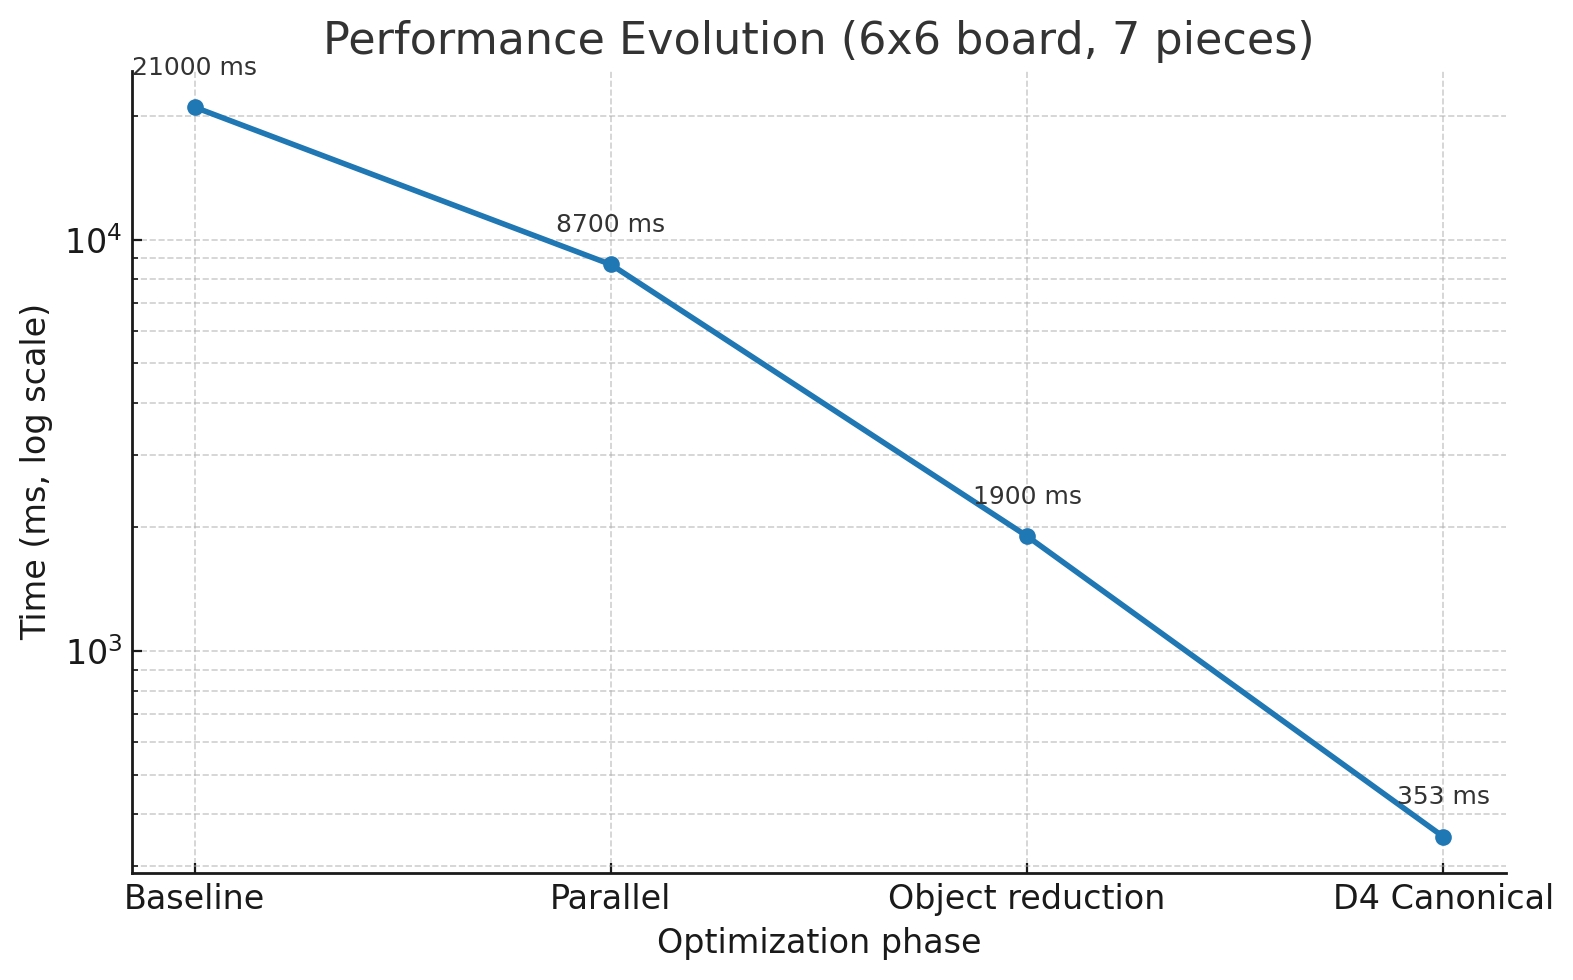
\includegraphics[width=0.75\textwidth]{performance_trend.png}
\caption{Performance evolution across optimization phases (6$\times$6 board). 
Logarithmic scale highlights exponential gap between baseline and symmetry elimination. 
Figure placeholder: replace with actual plot.}
\end{figure}

\section{Threats to Validity}

Despite extensive validation, several factors may affect results:

\begin{itemize}
\item \textbf{Hardware variability:} CPU turbo frequencies, OS scheduling and WSL overhead can cause small deviations.
\item \textbf{JVM effects:} Garbage collection and JIT optimizations may shift timings across runs.
\item \textbf{Symmetry assumptions:} While all 6$\times$6 solutions had orbit size 8, larger boards may contain partial symmetries, leading to smaller orbits.
\item \textbf{Algorithmic trade-offs:} Canonicalization at leaf-level avoids false negatives but may miss early pruning opportunities.
\end{itemize}

\section{Conclusion}

This case study demonstrates how systematic algorithmic optimization can transform computationally challenging problems into efficiently solvable ones, while also revealing fundamental limits through comprehensive exploration. The key breakthrough was recognizing that the chess piece placement problem exhibits group symmetries, allowing us to reduce the 6$\times$6 solution space by an order of magnitude while maintaining mathematical correctness.

---

\bibliographystyle{plain}
\begin{thebibliography}{99}

\bibitem{knuth1975}
D.E. Knuth, \emph{The Art of Computer Programming, Volume 4A: Combinatorial Algorithms}, Addison-Wesley, 2011.

\bibitem{russell2020}
S. Russell and P. Norvig, \emph{Artificial Intelligence: A Modern Approach}, 4th edition, Pearson, 2020.

\bibitem{garey1979}
M.R. Garey and D.S. Johnson, \emph{Computers and Intractability: A Guide to the Theory of NP-Completeness}, Freeman, 1979.

\bibitem{brualdi2010}
R.A. Brualdi, \emph{Introductory Combinatorics}, 5th edition, Pearson, 2010.

\bibitem{burnside1897}
W. Burnside, \emph{Theory of Groups of Finite Order}, Cambridge University Press, 1897.

\bibitem{scala2021}
M. Odersky et al., \emph{Programming in Scala}, 5th edition, Artima Press, 2021.

\end{thebibliography}

\end{document}
